\subsection{OWASP-ZAP Layout}

Nesta secção pretendemos explicar todos os recursos importantes disponibilizados pelo ZAP. E a configuração da interface do mesmo.


\subsubsection{Desktop UI Overview}

\paragraph{Top Level Menu}

Em primeiro lugar vamos referir as opções oferecidas pelo menu superior da aplicação. Este menu oferece acesso a praticamente todos os recursos do ZAP e não só isso como também permite configurar os mesmos.

\begin{itemize}
\item File menu\newline

\par Permite que possamos criar uma nova sessão, importar uma sessão guardada, apagar a sessão atual, guarda-la ou sair da aplicação.

\item Edit menu \newline

\par Permite mudar o modo em que o ZAP opera: 

- safe: não são realizadas operações potencialmente perigosas.

- protected: só podemos realizar operações potencialmente perigosas nos URLs especificados

- Standard: podemos realizar qualquer operação que o ZAP suporte

- ATTACK: novos nodos que entram na "mapa" resultados do spider do site são ativamente scaneados mal seja descobertos.

\par Permite manter o utilizador autenticado no site alvo com a opção \textit{forced user mode}.


\item View menu \newline

\par Permite ver a \textit{history tab}, que por sua vez mostra todos os pedidos feitos ordenados no tempo possuindo as informações de index, método HTML usado (GET/POST), URL, código de resposta HTTP, explicação do que significa o código anterior, o tempo que demorou o pedido, qualquer alerta de vulnerabilidade no pedido, notas adicionadas ao pedido e tags associadas ao mesmo.  


\item Analyse menu \newline

\par Este menu permite modificar uma politica de análise\footnote[1]{Uma politica de análise define um conjunto de regras a serem seguidas durante uma análise átiva. Também define quants pedidos são feitos e quão provável será potenciais problemas serem assinalados.} ou adicionar uma nova.


\item Report menu  \newline

\par permite gerar um relatórico com todos os alertas encontrados em formato HTML, XML ou Markdown.

\item Tools menu \newline

\par Este menu pemite aceder ás opções de configuração das ferramentas e recursos disponíveis no ZAP.
\begin{itemize}
\item Nas configurações de scan ativo podemos definir:\newline

\par - O número de hosts a serem analisados ao mesmo tempo;\newline

\par - Quantas threads existirão por host;\newline

\par - O nnúmero de resultados que aparecerão na tab do scan ativo;\newline

\par - O tempo máximo que uma regra da politica de análise poderá demorar;\newline

\par - O tempo máximo que um scan pode demorar;\newline

\par - O delay em (milisegundos) entre pedidos feitos;\newline

\par - Se queremos que seja injetado em cada pedido o identificador do mesmo no ZAP na forma X-ZAP-Scan-ID;\newline

\par - Se queremos que durante o scan o zap tente obter tokens anti CSRF\footnote[2]{OS tokens Anti CSRF são parâmetros pseudo aleatórios usados para proteção contra ataques de Cross Site Request Forgery (CSRF).};\newline

\par - Usar a definição padrão de análise ativa;\newline

\par - Usar a definição padrão de análise de ataque; \newline


\item Nos vetores de input do scan ativo podemos definir como inputs:

\par - Strings de URL específicas após o ?; \newline

\par - Pares chave-valor nos dados Post pedidos; \newline

\par - Elementos de caminhos URL; \newline

\par - Cabeçalhos HTTP; \newline

\par - Cookies; \newline

\item Podemos adicionalmente escolher o formato dos inputs do scan ativo sendo estes:

\begin{itemize}

\item Multipart Form Data	
\item XML tag/attribute	
\item JSON	
\item Google Web Toolkit	
\item OData id/filter

\end{itemize}

\item Podemos definir como queremos que os alertas nos sejam apresentados:

\par - Podemos reduzir o tamanho dos relatórios significativamente caso façamos merge de alertas iguais encontrados em pontos diferentes do scan.  \newline
\par - Podemos também escolher o número máximo de alertas que pretendemos que constem no relatório. \newline
\par - Por último é-nos dada a opão de modificar a mensagem associada com um alerta específico para melhor compreensão. \newline

\item Outro ponto configurável são os tokens anti CRSF, podemos escolher quais queremos analisar.

\item Podemos definir o endereço e a porta em que o ZAP vai ficar á escuta de conecções, caso não sejam definidos o ZAP usa o localhost como endereço e liga-se a uma porta aleatória disponível na máquina. 

\item O ZAP permite gerar um certificado SSL dinâmico para os casos em que as aplicações usem SSL mútuo.\newline
\par Para permitir conecções SSL trasparentes é necessário encriptar cada pedido feito ao servidor e desencriptar cada reposta do mesmo, como o browser usado já faz isso, a única maneira de o ZAP fazer isto é atrvés de um ataque "man-in-the-middle". Para isto basta que adicionemos aos certificados de confiança do browser escolhido o ZAP Root CA certificate. Desta forma como o ZAP cria um certificado assinado para cada servidor sobre o qual realiza o ataque "man-in-the-middle", usar o ZAP Root CA certificate é uma forma de assegurar ao browser que pode confiar nesse certificado.

\item O ZAP também permite definir e configurar o tipo de conecção a ser usada:

\par - Podemos definir um timeout que o que facilita o teste de aplicações lentas.\newline
\par - Podemos definir o utilizador que o ZAP deve sar ao criar asa mensagens HTTP.\newline
\par - Podemos definir se o ZAP usa um "Single cookie request header" ou "multiple cookie request header"\footnote[3]{O Cookie HTTP request header contem cookies HTTP enviadas previamente em respostas do servidor, o Zap possibilita enviar as cookies todas juntas ou uma de cada vez por HTTP request header.}.\newline
\par - Podemos ativar o (Global) HTTP State, isto é, podemos rastrear as cookies guardadas na sessão.\newline
\par - Podemos definir por quanto tempo as queries DNS bem sucedidas devem ser guardadas em cache (números negativos represetam sem limite de tempo, zero não permite guardar e números positivos representam o tempo em segundos a guardar).\newline
\par - Podemos ainda definir as versões dos protocolos a usar nas conecções efetuadas. Devemos no entanto ter a opção "SSLv2Hello" selecionadacom pelo menos uma versão de SSL/TLS. \newline


\item Podemos também definir vários regex para URLs que o ZAP irá ignorar. Estes regex podem ser ainda modificados ou removidos.
\end{itemize}

\item Help menu \newline


\par - Neste menu podemos procurar ajuda sobre como utilizar o ZAP, procurar ajuda para resolver problemas de versões do ZAP e add-ons e para verificar a existencia de updates.\newline

\end{itemize}

\paragraph{Toolbar Menu} \hfill\newline
\hfill\newline
\par Neste menu podemos encontrar formas de dispor o layout do ZAP para que se torne mais agradável á vista ou para podermos visualizar vários paineis úteis simultaneamente. Neste menu destacam-se algumas features que achamos interessantes nomeadamente:\newline

\begin{figure}[H]

  \centering

  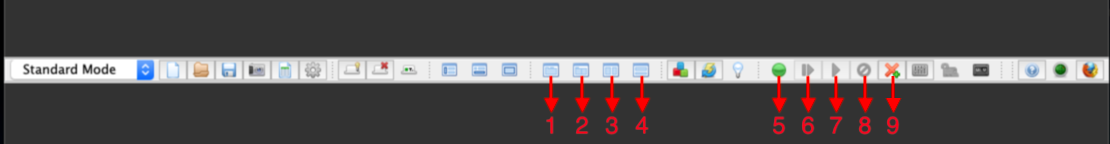
\includegraphics[scale = 0.31]{fig18.png}

  \caption{Toolbar Menu}

\end{figure}

\par Neste menu podemos definir se queremos colocar os pedidos feitos ao servidor e as respetivas respostas ao servidor lado a lado. Para isso temos 2 opções disponíveis.


\begin{enumerate}

\item Colocar os pedidos e respostas em tabs lado a lado.
\item Colocar os pedidos e respostas na mesma tab lado a lado.
\item Colocar os pedidos na parte esquerda de uma tab e as respetivas respostas na direita.
\item Colocar os pedidos na parte superior de uma tab e as respetivas respostas na inferior.

\par Adicionalmente este menu permite um controlo maior sobre os pedidos e as respostas do servidor, permitindo-nos adicionar um break em cada pedido, resposta ou nos dois e modificar os pedidos, evitar que um pedido seja feito ou remover um par pedido-resposta. O botão usado para implementar os breaks é  o circulo assinalado pelo número 5.\newline

\par Possuimos também auxiliares para trabalhar com os breakpoints assinalados com os números 6,7,e 8 que executam as seguintes ações sobre os pedidos e respostas apanhadas respetivamente saltar para o próximo par pedido resposta, continuar a realizar os pedidos e respostas e parar apenas no caso de termos definido um breakpoint para um URL específico\footnote[4]{Um breakpoint pode ser definido para um URL especifico com recurso ao elemento identifocado como 9.} e destruir o par pedido-resposta apanhado pelo breakpoint. \newline
\end{enumerate}

\paragraph{Windows} \hfill\newline
\hfill\newline
\begin{enumerate}

\item Sites Window, nesta podemos ver toda a informação referente aos sites que visitamos, isto inclui o URL, pedidos GET associados ao URL, pastas ocultas encontradas neste entre outros.

\begin{figure}[H]

  \centering

  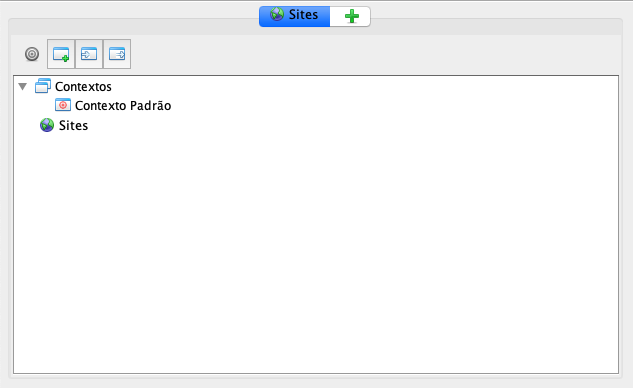
\includegraphics[scale = 0.31]{fig19.png}

  \caption{Sites Window}

\end{figure}

\item Workspace Window, nesta podemos visualizar as informações dos pedidos e as respetivas respostas. Também é nesta janela que podemos efetuar alterações aos mesmos quando temos breakpoints definidos.

\begin{figure}[H]

  \centering

  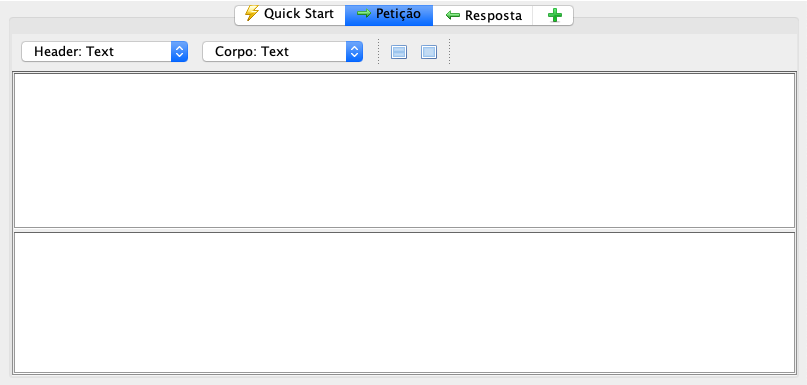
\includegraphics[scale = 0.31]{fig20.png}

  \caption{Workspace Window}

\end{figure}

\item Information Window, nesta última janela encontramos todas as informações úteis referentes aos testes de segurança realizados sobre um site. As informações estão organizadas nas seguintes tabs:
\begin{itemize}
	\item History tab: Mostra os pedidos pela ordem em que foram feitos, permitindo modificar a ordem pelo atributo que o utilizador quiser (url, método, código, alerta mais importante,...).
	\item Search tab: Permite uma pesquisa entre todos os pedidos e respostas de um teste.

	\item Breakpoints tab: mostra os breakpoints feitos num teste.

	\item Alerts tab: Mostra todos os alertas encontrados na aplicação durante o teste.

	\item Active Scan tab: Mostra os scans ativos 

	\item Spider tab: Mostra os URLs que ainda não foram visitados

	\item Params tab: Mostra um sumário dos parâmetros que um site utiliza.

	\item Output tab: Mostra várias mensagens informativas sobre o teste realizado.

	\item Callbacks tab: Mostra pedidos de callbacks que o ZAP recebeu durante os testes ao site.

\end{itemize}
\begin{figure}[H]

  \centering

  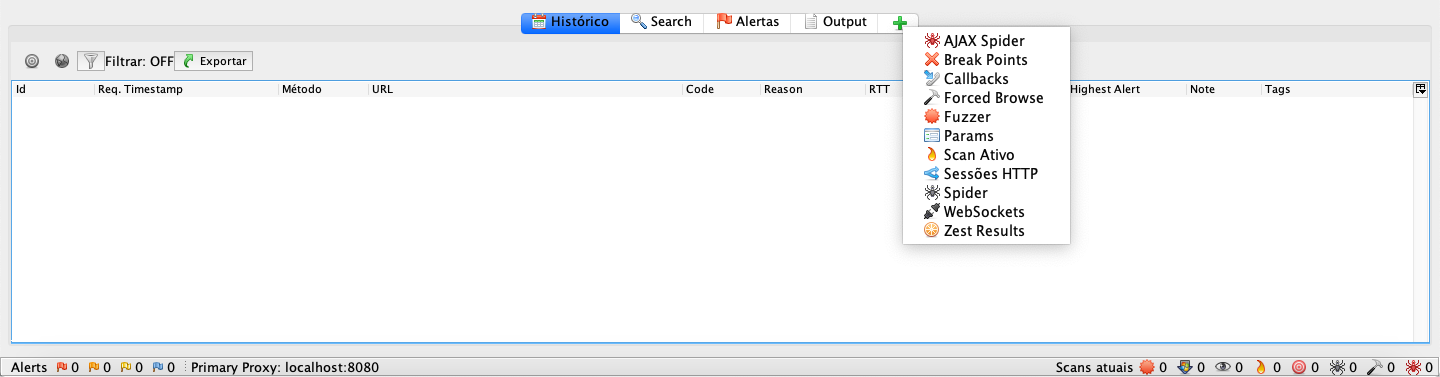
\includegraphics[scale = 0.31]{fig21.png}

  \caption{Information Window}

\end{figure}
\end{enumerate}
